
\begin{figure}[!ht]
    \centering
    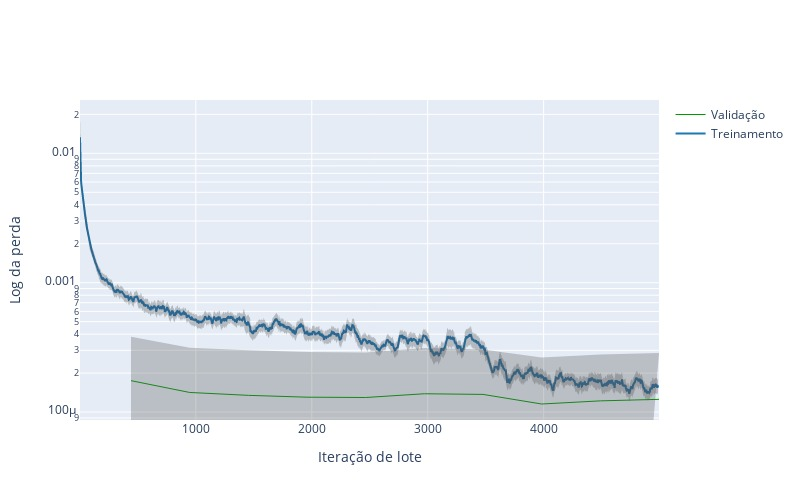
\includegraphics[width=\columnwidth]{Imagens/results/rsp-swin-t_planet_pt/Training Loss Per Minibatch.jpg}
    \caption{ Arquitetura de modelo base. Fonte: Autor}
    \label{fig:LossTrainSwin}
\end{figure}

\begin{figure}[!ht]
    \centering
    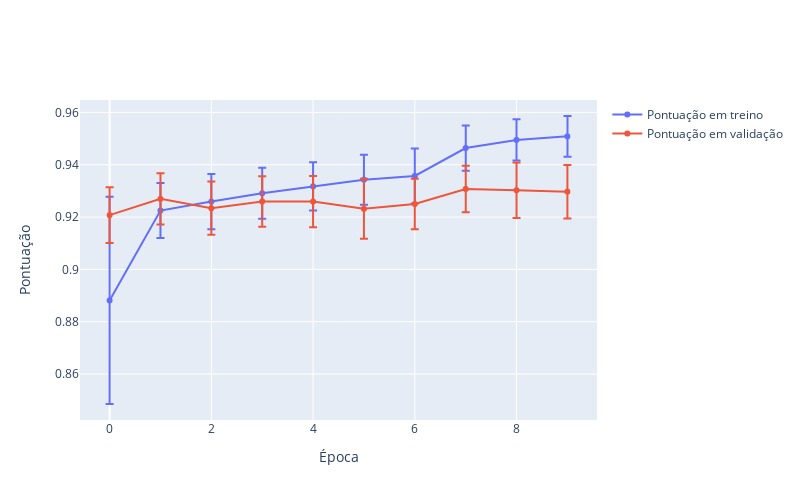
\includegraphics[width=\columnwidth]{Imagens/results/rsp-swin-t_planet_pt/pontuação em treino e validação por época.jpg}
    \caption{ Arquitetura de modelo base.Fonte: Autor}
    \label{fig:PontuacaoTrainSwin}
\end{figure}  
\begin{figure}[!ht]
    \centering
    \includegraphics[width=\columnwidth]{Imagens/results/rsp-swin-t_planet_pt/Inferência para cada classe.jpg}
    \caption{ Arquitetura de modelo base.
    Fonte: Autor}
    \label{fig:InferenciaClassesSwin}
\end{figure}  



\begin{figure}[!ht]
    \centering
    \includegraphics[width=\columnwidth]{Imagens/results/rsp-swin-t_planet_pt/Matrizes confusão.jpg}
    \caption{ Matriz Confusão SwinT. Fonte: Autor}
    \label{fig:Matriz Confusao SwinT}
\end{figure}  

\begin{figure}[!ht]
    \centering
    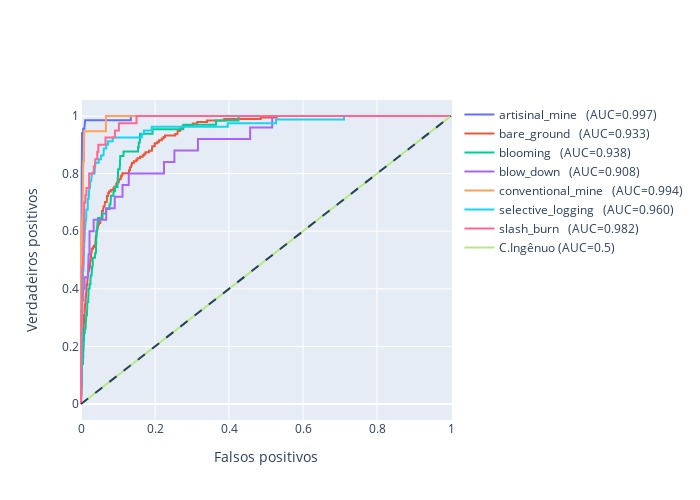
\includegraphics[width=\columnwidth]{Imagens/results/rsp-swin-t_planet_pt/Curva COR para classes raras.jpg}
    \caption{ Curva COR.
    Fonte: Autor}
   \label{fig:AnexosCurvaCORResnet50}
\end{figure}    

\begin{figure}[!ht]
    \centering
    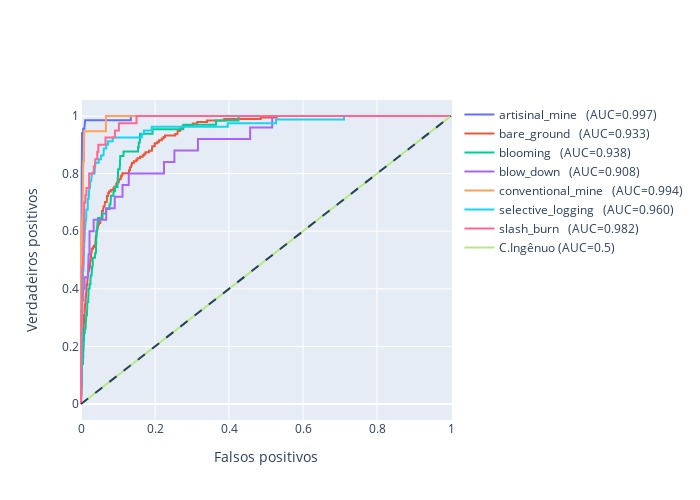
\includegraphics[width=\columnwidth]{Imagens/results/rsp-swin-t_planet_pt/Curva COR para classes raras.jpg}        
    \caption{ Curva COR.
    Fonte: Autor}
   \label{fig:AnexosCurvaCORSwint}
\end{figure}    

\begin{figure}[!ht]
    \centering
    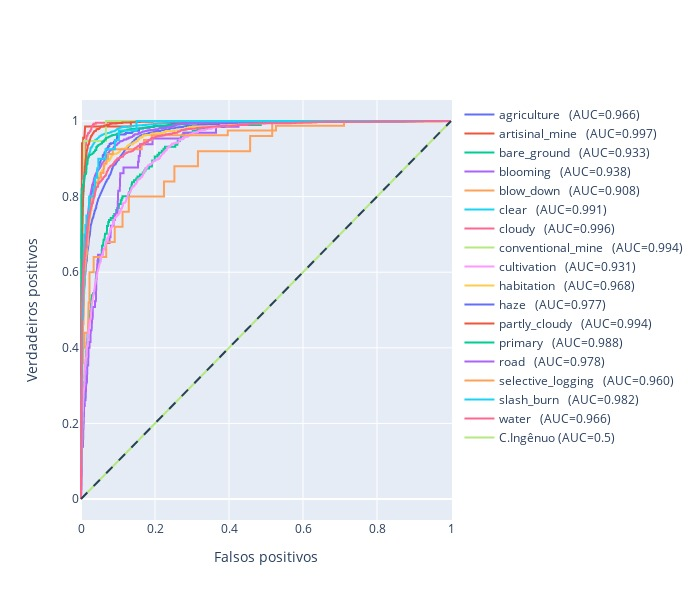
\includegraphics[width=\columnwidth]{Imagens/results/rsp-swin-t_planet_pt/Curva COR por classe.jpg}
    \caption{ Curva COR.
    Fonte: Autor}
    \label{fig:AnexosCurvaCORTodasSwin}
\end{figure}    

\begin{figure}[!ht]
    \centering
    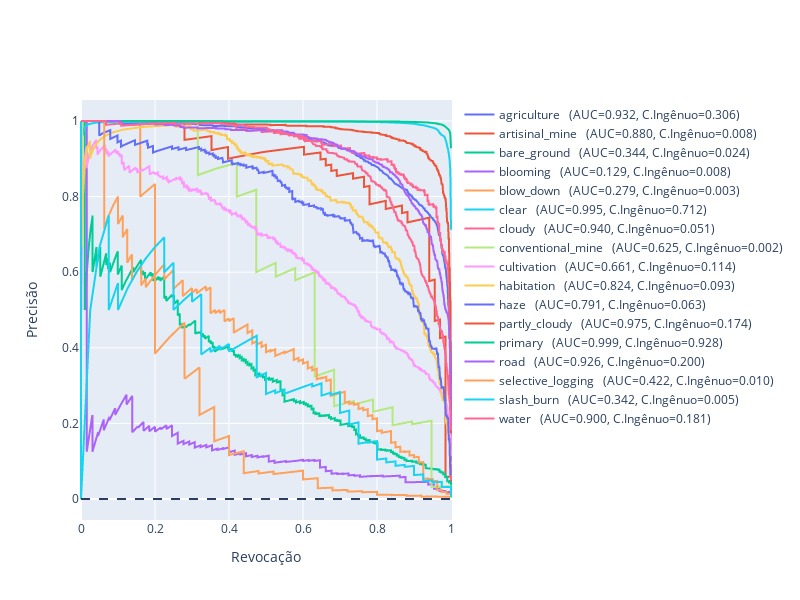
\includegraphics[width=\columnwidth]{Imagens/results/rsp-swin-t_planet_pt/Curva PR por classe.jpg}
    \caption{ Arquitetura de modelo base.
    Fonte: Autor}
    \label{fig:AnexosCurvaPRTodasSwin}
\end{figure}  



\begin{table}[h!]
    \caption{Resultados do Modelo Swin-T}
    \centering
\begin{tabular}{*{6}{c}}
    \toprule
    {} &              label &  F2    &  threshold &  PR AUC &  PR-AUC Class.Ingênuo \\
    \midrule
    3  &           blooming &  0,230 &      0,270 &   0,129 &       0,008 \\
    4  &          blow down &  0,310 &      0,190 &   0,279 &       0,003 \\
    15 &         slash burn &  0,338 &      0,130 &   0,342 &       0,005 \\
    2  &        bare ground &  0,447 &      0,170 &   0,344 &       0,024 \\
    14 &  selective logging &  0,475 &      0,110 &   0,422 &       0,010 \\
    7  &  conventional mine &  0,538 &      0,210 &   0,625 &       0,002 \\
    8  &        cultivation &  0,681 &      0,130 &   0,661 &       0,114 \\
    9  &         habitation &  0,780 &      0,390 &   0,824 &       0,093 \\
    10 &               haze &  0,787 &      0,230 &   0,791 &       0,063 \\
    16 &              water &  0,830 &      0,250 &   0,900 &       0,181 \\
    13 &               road &  0,865 &      0,190 &   0,926 &       0,200 \\
    1  &     artisinal mine &  0,872 &      0,250 &   0,880 &       0,008 \\
    0  &        agriculture &  0,889 &      0,290 &   0,932 &       0,306 \\
    6  &             cloudy &  0,907 &      0,270 &   0,940 &       0,051 \\
    11 &      partly cloudy &  0,942 &      0,170 &   0,975 &       0,174 \\
    5  &              clear &  0,978 &      0,190 &   0,995 &       0,712 \\
    12 &            primary &  0,991 &      0,230 &   0,999 &       0,928 \\
    17 &             global &  0,930 &      0,216 &   0,704 &       0,170 \\
    \bottomrule
\end{tabular}
\label{table:AnexosResultadosSwinT}
\end{table}


\begin{table}[h!]
    \caption{Resultados do Modelo ResNet50}
    \centering
\begin{tabular}{*{6}{c}}
    \toprule
    {} &              label &  F2    &  threshold &  PR AUC &  PR-AUC Class.Ingênuo \\
    \midrule
    15 &         slash burn &  0,030 &      0,230 &   0,145 &       0,005 \\
    3  &           blooming &  0,140 &      0,130 &   0,096 &       0,008 \\
    4  &          blow down &  0,268 &      0,190 &   0,245 &       0,003 \\
    2  &        bare ground &  0,373 &      0,210 &   0,316 &       0,024 \\
    14 &  selective logging &  0,422 &      0,090 &   0,401 &       0,010 \\
    7  &  conventional mine &  0,579 &      0,170 &   0,536 &       0,002 \\
    8  &        cultivation &  0,674 &      0,130 &   0,650 &       0,114 \\
    9  &         habitation &  0,769 &      0,130 &   0,802 &       0,093 \\
    10 &               haze &  0,774 &      0,210 &   0,784 &       0,063 \\
    16 &              water &  0,836 &      0,210 &   0,892 &       0,181 \\
    1  &     artisinal mine &  0,840 &      0,190 &   0,880 &       0,008 \\
    13 &               road &  0,864 &      0,210 &   0,916 &       0,200 \\
    0  &        agriculture &  0,890 &      0,250 &   0,929 &       0,306 \\
    6  &             cloudy &  0,910 &      0,230 &   0,946 &       0,051 \\
    11 &      partly cloudy &  0,938 &      0,210 &   0,972 &       0,173 \\
    5  &              clear &  0,978 &      0,210 &   0,996 &       0,713 \\
    12 &            primary &  0,992 &      0,190 &   0,999 &       0,928 \\
    17 &             global &  0,928 &      0,188 &   0,677 &       0,170 \\
    \bottomrule
\end{tabular}
\label{table:AnexosResultadosResnet50}
\end{table}    
